\documentclass{beamer}
\usepackage[utf8]{inputenc}

\usetheme{Madrid}
\usecolortheme{default}
\usepackage{amsmath,amssymb,amsfonts,amsthm}
\usepackage{txfonts}
\usepackage{tkz-euclide}
\usepackage{listings}
\usepackage{adjustbox}
\usepackage{array}
\usepackage{tabularx}
\usepackage{gvv}
\usepackage{lmodern}
\usepackage{circuitikz}
\usepackage{tikz}
\usepackage{graphicx}
\usepackage{gensymb}

\setbeamertemplate{page number in head/foot}[totalframenumber]

\usepackage{tcolorbox}
\tcbuselibrary{minted,breakable,xparse,skins}



\definecolor{bg}{gray}{0.95}
\DeclareTCBListing{mintedbox}{O{}m!O{}}{%
  breakable=true,
  listing engine=minted,
  listing only,
  minted language=#2,
  minted style=default,
  minted options={%
    linenos,
    gobble=0,
    breaklines=true,
    breakafter=,,
    fontsize=\small,
    numbersep=8pt,
    #1},
  boxsep=0pt,
  left skip=0pt,
  right skip=0pt,
  left=25pt,
  right=0pt,
  top=3pt,
  bottom=3pt,
  arc=5pt,
  leftrule=0pt,
  rightrule=0pt,
  bottomrule=2pt,
  toprule=2pt,
  colback=bg,
  colframe=orange!70,
  enhanced,
  overlay={%
    \begin{tcbclipinterior}
    \fill[orange!20!white] (frame.south west) rectangle ([xshift=20pt]frame.north west);
    \end{tcbclipinterior}},
  #3,
}
\lstset{
    language=C,
    basicstyle=\ttfamily\small,
    keywordstyle=\color{blue},
    stringstyle=\color{orange},
    commentstyle=\color{green!60!black},
    numbers=left,
    numberstyle=\tiny\color{gray},
    breaklines=true,
    showstringspaces=false,
}
\begin{document}

\title 
{4.11.12}
\date{September 27,2025}


\author 
{Kishora Karthik-EE25BTECH11034}
\frame{\titlepage}
\begin{frame}{Question}
Find the distance of the point $P(-1,-5,-10)$ from the point of intersection of the line
$\vec{r} = 2\hat{\imath}-\hat{\jmath}+2\hat{k}+\lambda\,(3\hat{\imath}+4\hat{\jmath}+2\hat{k})$
and the plane
$\vec{r}\cdot(\hat{\imath}-\hat{\jmath}+\hat{k})=5$.
\\
\end{frame}

\begin{frame}{ Solution}
The line is given by $\vec{x}=\vec{h}+k\vec{m}$, where 
\begin{align}
    \vec{x}=\myvec{2\\-1\\2}
\end{align}
\begin{align}
    \vec{m}=\myvec{3\\4\\2}
\end{align}
The plane is of the form $\vec{n}^\top\vec{x}=c$ where $c=5$ and,
\begin{align}
\vec{n}=\myvec{1\\-1\\1}
\end{align}
Given, $\vec{P}=\myvec{-1\\-5\\-10}$.
\end{frame}

\begin{frame}{Solution}
To find the point of intersection, we substitute the vector equation of the line into the vector equation of the plane.
\begin{align}
(\vec{a} + \lambda\vec{b}) \cdot \vec{n} = c
\end{align}
\begin{align}
\vec{h} \cdot \vec{n} + k(\vec{m} \cdot \vec{n}) = c
\end{align}
\begin{align}
\vec{h}  \vec{n}^\top + k(\vec{m} \vec{n}^\top) = c
\end{align}
\begin{align}
\myvec{2\\-1\\2} \cdot \myvec{1&-1&1} + k\myvec{3\\4\\2} \cdot \myvec{1&-1&1} = 5
\end{align}
\end{frame}
\begin{frame}{Solution}
\begin{align}
(2\cdot1+(-1)\cdot(-1)+(2)\cdot(1))+k(3\cdot1+4\cdot(-1)+2\cdot(1)) = 5    
\end{align}
\begin{align}
    (5)+k(1) = 5
\end{align}
\begin{align}
    k = 0
\end{align}
The point of intersection is $\vec{x} = \vec{h} + 0(\vec{m}) = \vec{h} $.
\end{frame}
\begin{frame}{Solution}
    Distance between two points is given by 
$\norm{\vec{x_2}-\vec{x_1}}$.\\
\begin{align}
    d=\norm{\myvec{-1\\-5\\-10}-\myvec{2\\-1\\2}}
\end{align}
\begin{align}
    d=\norm{\myvec{-3\\-4\\12}}
\end{align}
\begin{align}
    d=\sqrt{(-3)^2+(-4)^2+(12)^2}
\end{align}
\begin{align}
    d=\sqrt{169}
\end{align}
\begin{align}
    d=13
\end{align}
$\therefore$ The distance between the points is 13 units.
\end{frame}
\begin{frame}{Plot}
    \centering
    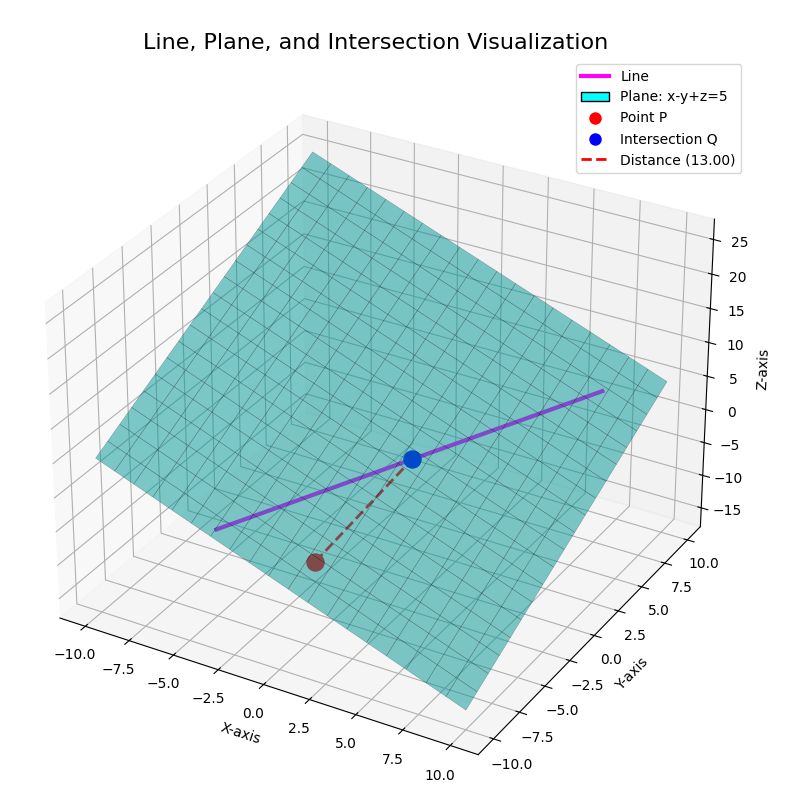
\includegraphics[width=\columnwidth, height=0.8\textheight, keepaspectratio]{figs/fig1.png} 
\end{frame}

\end{document}




